% -----------------------------------------------
% Template for ISMIR Papers
% 2021 version, based on previous ISMIR templates

% Requirements :
% * 6+n page length maximum
% * 10MB maximum file size
% * Copyright note must appear in the bottom left corner of first page
% * Clearer statement about citing own work in anonymized submission
% (see conference website for additional details)
% -----------------------------------------------

\documentclass{article}
\usepackage[T1]{fontenc} % add special characters (e.g., umlaute)
\usepackage[utf8]{inputenc} % set utf-8 as default input encoding
\usepackage{ismir,amsmath,cite,url}
\usepackage{graphicx}
\usepackage{color}


\usepackage{lineno}
\linenumbers

% Title. Please use IEEE-compliant title case when specifying the title here,
% as it has implications for the copyright notice
% -----
\title{Revisiting "Shallow" Music Representation Learning with HDPGMM}

% Note: Please do NOT use \thanks or a \footnote in any of the author markup

% Single address
% To use with only one author or several with the same address
% ---------------
%\oneauthor
% {Names should be omitted for double-blind reviewing}
% {Affiliations should be omitted for double-blind reviewing}

% Two addresses
% --------------
%\twoauthors
%  {First author} {School \\ Department}
%  {Second author} {Company \\ Address}

% Three addresses
% --------------\input{ISMIR2021_paper.tex}

\threeauthors
  {First Author} {Affiliation1 \\ {\tt author1@ismir.edu}}
  {Second Author} {\bf Retain these fake authors in\\\bf submission to preserve the formatting}
  {Third Author} {Affiliation3 \\ {\tt author3@ismir.edu}}

% Four or more addresses
% OR alternative format for large number of co-authors
% ------------
%\multauthor
%{First author$^1$ \hspace{1cm} Second author$^1$ \hspace{1cm} Third author$^2$} { \bfseries{Fourth author$^3$ \hspace{1cm} Fifth author$^2$ \hspace{1cm} Sixth author$^1$}\\
%  $^1$ Department of Computer Science, University , Country\\
%$^2$ International Laboratories, City, Country\\
%$^3$  Company, Address\\
%{\tt\small CorrespondenceAuthor@ismir.edu, PossibleOtherAuthor@ismir.edu}
%}

% For the author list in the Creative Common license, please enter author names. 
% Please abbreviate the first names of authors and add 'and' between the second to last and last authors.
\def\authorname{F. Author, S. Author, and T. Author}

% Optional: To use hyperref, uncomment the following.
%\usepackage[bookmarks=false,pdfauthor={\authorname},pdfsubject={\papersubject},hidelinks]{hyperref}
% Mind the bookmarks=false option; bookmarks are incompatible with ismir.sty.

\sloppy % please retain sloppy command for improved formatting

\begin{document}

%
\maketitle
%
\begin{abstract}
The abstract should be placed at the top left column and should contain about 150-200 words.
\end{abstract}
%
\section{Introduction}\label{sec:introduction}

blah blah
%

\section{Related works}\label{sec:rel_works}

blah blah
%
\section{HDPGMM}\label{sec:hdpgmm}

In this subsection, we introduce the main model we employ for this study; the Hiararchical Dirichlet Process Gaussian Mixture Model (HDPGMM). To introduce the model properly it would be useful to start discussing the Dirichlet Process Mixture Model (DPMM), the model on which HDPGMM is extended.

\subsection{Dirichlet Process Mixture Models}

Mixture models such as GMMs assumes a finite number of components from which each of observed feature vectors are drawn. It is well known that finding the optimal number $K$ of the mixuture components is a difficult problem. There are a few approaches that can be useful to estimate $K$, for instance, using the cross-validation. Dirichlet Process Mixture Model (DPMM) circumbents this problem by parametrizing the number of mixtures as part of the model. DP plays a central role for such models.

DP is a stochastic process which draws random probability distributions. Due to this property, it is often described as a distribution over distributions \cite{DBLP:reference/ml/Teh17}. Another important characteristic of DP is that it assumes the existence of a countable infinite number of mixtures components while only a finite subset of them are emerged from the observations~\cite{DBLP:reference/ml/Teh17}. This aspect is the core building block of the Bayesian non-parametric models such as infinite mixture models. Setting DP as a prior distribution for the responsibility $\pi$ (also often referred as mixture probability) of mixture components allows the mixture model to infer both the relative weight among components and the appropriate number of maximum components for given observations.

Among a several ways to represent DP, we introduce the Stick-Breaking construction~\cite{sethuraman94}.
\footnote{Literature commonly chooses the Chinese Restaurant Process (CRP) for a illustrative metaphor for DP as it is intuitive and well explains various properties of DP~\cite{DBLP:reference/ml/Teh17}. We mainly discuss DP with the stick-breaking construction due to its further usage in the model inference within the work. For readers interested in other metaphorical descriptions of DP, we kindly refer them to~\cite{DBLP:reference/ml/Teh17, DBLP:conf/ismir/HoffmanBC08}}
Stick-breaking constructs DP in a simple and general manner. Formally, it is as follows:

\begin{equation}
\begin{aligned}[c]
    \beta^{\prime}_{k} &\sim \text{Beta}(1, \gamma) \\
    \beta_{k} &= \beta^{\prime}_{k} \prod_{l=1}^{k-1} (1 - \beta_{l}^{\prime}) \\
\end{aligned}
\qquad\qquad
\begin{aligned}[c]
    \phi_{k} &\sim H \\
    G_{0} &= \sum^{\infty}_{k=1} \beta_{k}\delta_{\phi_{k}}
\end{aligned}
\end{equation}



\section{Page Size}\label{sec:page_size}

The proceedings will be printed on
 \underline{portrait A4-size paper} \underline{(21.0cm x 29.7cm)}.
All material on each page should fit within a rectangle of 17.2cm x 25.2cm,
centered on the page, beginning 2.0cm
from the top of the page and ending with 2.5cm from the bottom.
The left and right margins should be 1.9cm.
The text should be in two 8.2cm columns with a 0.8cm gutter.
All text must be in a two-column format.
Text must be fully justified.

\section{Typeset Text}\label{sec:typeset_text}

\subsection{Normal or Body Text}\label{subsec:body}

Please use a 10pt (point) Times font. Sans-serif or non-proportional fonts
can be used only for special purposes, such as distinguishing source code text.

The first paragraph in each section should not be indented, but all other paragraphs should be.

\subsection{Title and Authors}

The title is 14pt Times, bold, caps, upper case, centered.
\textcolor{red}{Authors' names are omitted when submitting for double-blind reviewing.}
The following is for making a camera-ready version.
Authors' names are centered.
The lead author's name is to be listed first (left-most), and the co-authors' names after.
If the addresses for all authors are the same, include the address only once, centered.
If the authors have different addresses, put the addresses, evenly spaced, under each authors' name.

\subsection{First Page Copyright Notice}

Please include the copyright notice exactly as it appears here in the lower left-hand corner of the page.
It is set in 8pt Times. \textcolor{red}{After your paper is accepted, you will need to insert the appropriate author names and paper title in the copyright notice when submitting the camera-ready version.} For \LaTeX users, this will be handled by the template automatically. For Word users, this has to be done manually.


\subsection{Page Numbering, Headers and Footers}

Do not include headers, footers or page numbers in your submission.
These will be added when the publications are assembled.

\subsection{Line Numbers}

Line numbers should be included in your originally submitted manuscript, for reference during reviewing. \textcolor{red}{However, after your paper is accepted, you must remove all line numbers from the final camera-ready version.} This can be done in \LaTeX by commenting out the command \verb|\linenumbers| on Line 22. This can be done in Microsoft Word by selecting Layout > Line Numbers > None.

\section{First Level Headings}

First level headings are in Times 10pt bold,
centered with 1 line of space above the section head, and 1/2 space below it.
For a section header immediately followed by a subsection header, the space should be merged.

\subsection{Second Level Headings}

Second level headings are in Times 10pt bold, flush left,
with 1 line of space above the section head, and 1/2 space below it.
The first letter of each significant word is capitalized.

\subsubsection{Third and Further Level Headings}

Third level headings are in Times 10pt italic, flush left,
with 1/2 line of space above the section head, and 1/2 space below it.
The first letter of each significant word is capitalized.

Using more than three levels of headings is highly discouraged.

\section{Footnotes and Figures}

\subsection{Footnotes}

Indicate footnotes with a number in the text.\footnote{This is a footnote.}
Use 8pt type for footnotes. Place the footnotes at the bottom of the page on which they appear.
Precede the footnote with a 0.5pt horizontal rule.

\subsection{Figures, Tables and Captions}

All artwork must be centered, neat, clean, and legible.
All lines should be very dark for purposes of reproduction and art work should not be hand-drawn.
The proceedings are not in color, and therefore all figures must make sense in black-and-white form.
Figure and table numbers and captions always appear below the figure.
Leave 1 line space between the figure or table and the caption.
Each figure or table is numbered consecutively. Captions should be Times 10pt.
Place tables/figures in text as close to the reference as possible.
References to tables and figures should be capitalized, for example:
see \figref{fig:example} and \tabref{tab:example}.
Figures and tables may extend across both columns to a maximum width of 17.2cm.

\begin{table}
 \begin{center}
 \begin{tabular}{|l|l|}
  \hline
  String value & Numeric value \\
  \hline
  Hello ISMIR  & \conferenceyear \\
  \hline
 \end{tabular}
\end{center}
 \caption{Table captions should be placed below the table.}
 \label{tab:example}
\end{table}

\begin{figure}
 \centerline{\framebox{
 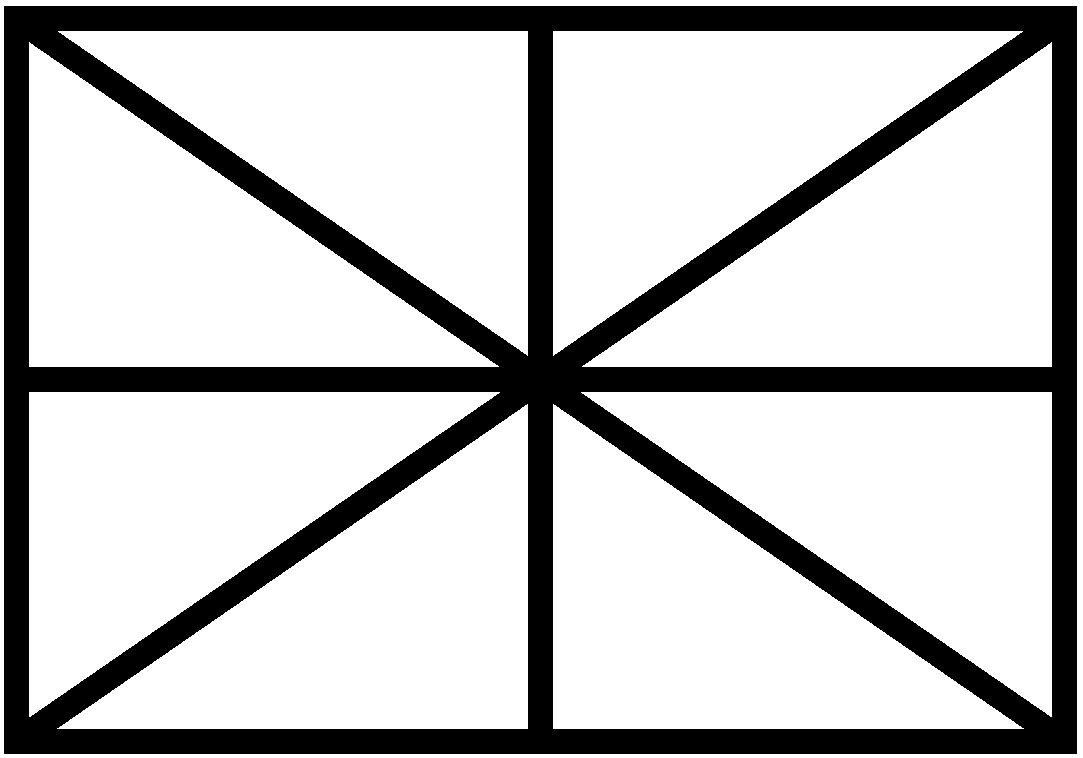
\includegraphics[width=0.9\columnwidth]{figure.png}}}
 \caption{Figure captions should be placed below the figure.}
 \label{fig:example}
\end{figure}

\section{Equations}

Equations should be placed on separate lines and numbered.
The number should be on the right side, in parentheses, as in \eqnref{relativity}.

\begin{equation}\label{relativity}
E=mc^{2}
\end{equation}

\section{Citations}

All bibliographical references should be listed at the end of the submission, in a section named ``REFERENCES,''
numbered and in the order that they first appear in the text. Formatting in the REFERENCES section must conform to the
IEEE standard (\url{https://ieeeauthorcenter.ieee.org/wp-content/uploads/IEEE-Reference-Guide.pdf}). Approved
IEEE abbreviations (Proceedings $\rightarrow$ Proc.) may be used to shorten reference listings. All references listed
should be cited in the text. When referring to documents, place the numbers in square brackets (e.g., \cite{ISMIR17Author:01}
for a single reference, or \cite{JNMR10Someone:01,Book20Person:01,Chapter09Person:01} for a range).

\textcolor{red}{As submission is double blind, refer to your own published work in the third person. That is, use ``In the previous work of \cite{ISMIR17Author:01},'' not ``In our previous work \cite{ISMIR17Author:01}.'' If you cite your other papers that are not widely available (e.g., a journal paper under review), use anonymous author names in the citation, e.g., an author of the form ``A. Anonymous.''}

% For bibtex users:
\bibliography{ISMIRtemplate}

% For non bibtex users:
%\begin{thebibliography}{citations}
% \bibitem{Author:17}
% E.~Author and B.~Authour, ``The title of the conference paper,'' in {\em Proc.
% of the Int. Society for Music Information Retrieval Conf.}, (Suzhou, China),
% pp.~111--117, 2017.
%
% \bibitem{Someone:10}
% A.~Someone, B.~Someone, and C.~Someone, ``The title of the journal paper,''
%  {\em Journal of New Music Research}, vol.~A, pp.~111--222, September 2010.
%
% \bibitem{Person:20}
% O.~Person, {\em Title of the Book}.
% \newblock Montr\'{e}al, Canada: McGill-Queen's University Press, 2021.
%
% \bibitem{Person:09}
% F.~Person and S.~Person, ``Title of a chapter this book,'' in {\em A Book
% Containing Delightful Chapters} (A.~G. Editor, ed.), pp.~58--102, Tokyo,
% Japan: The Publisher, 2009.
%
%
%\end{thebibliography}

\end{document}

